\documentclass[11pt]{article}
\usepackage[margin=0.88in]{geometry}
\usepackage[T1]{fontenc}
\usepackage{lmodern}
\usepackage{microtype}
\usepackage{amsmath,amssymb,amsthm,mathtools}
\usepackage{booktabs,array}
\usepackage{float}
\usepackage{xcolor}
\usepackage{graphicx}
\usepackage{tikz}
\usepackage[colorlinks=true,linkcolor=blue!55!black,urlcolor=blue!55!black,citecolor=blue!55!black]{hyperref}

\definecolor{accent}{RGB}{33,92,130}
\definecolor{soft}{RGB}{236,244,248}
\newtheorem{theorem}{Theorem}
\newtheorem{lemma}{Lemma}
\newcommand{\Ext}{\operatorname{Ext}}
\newcommand{\conv}{\operatorname{conv}}
\newcommand{\Lop}{\mathcal L}

\title{A Rational-Octagon Counterexample to Necessity\\
of the Weak Lindenstrauss--Perles Vertex Count}
\author{Automated mathematical discovery packet for arXiv:2006.15318\\
\small model: GPT5.6; lane: agent\_lane\_08}
\date{19 July 2026}

\begin{document}
\maketitle

\begin{abstract}
Mal, Paul, and Dey proved a vertex-count condition sufficient for a pair of
finite-dimensional polygonal Banach spaces to have weak
Lindenstrauss--Perles property. They proved necessity for a particular
two-dimensional range and left necessity for arbitrary polygonal planes
open. We give a negative answer. Let $X$ be the polygonal plane whose unit
ball is the rational octagon with vertices
\[
 \pm(1,0),\quad \pm(2/3,2/3),\quad \pm(0,1),\quad
 \pm(-2/3,2/3).
\]
Then every extreme contraction $T:X\to X$ maps some vertex of $B_X$ to a
vertex of $B_X$, although $B_X$ has eight vertices and fails the proposed
strict count. The proof is a complete exact classification of the
four-dimensional rational operator polytope: its 96 vertices form six
signed-permutation orbits, each with an explicit vertex-to-vertex witness.
\end{abstract}

\section{Source question and answer}

A pair $(X,Y)$ has \emph{weak L-P property} if every extreme point
$T$ of the operator unit ball $B_{\Lop(X,Y)}$ satisfies
\[
 T(\Ext B_X)\cap \Ext B_Y\ne\varnothing.
\]
The source's Theorem 2.5 says that if $\dim X=n$, $\dim Y=m$, and
$|\Ext B_X|=2(n+p)$, then
\[
 mp<n+p \tag{1}
\]
is sufficient for weak L-P property. After proving necessity in one special
two-dimensional range and constructing pair-dependent failures, the authors
state that necessity for arbitrary polygonal planes is not known.

\begin{center}

\includegraphics[width=0.96\textwidth]{figures/open_problem_crop.png}
\end{center}

\begin{theorem}[Negative answer to necessity]\label{thm:main}
Let
\[
 V_+=\left\{(1,0),\left(\frac23,\frac23\right),(0,1),
 \left(-\frac23,\frac23\right)\right\},\qquad
 B=\conv(V_+\cup -V_+),
\]
and let $X=(\mathbb R^2,\|\cdot\|_B)$. Then $(X,X)$ has weak L-P
property. On the other hand, $|\Ext B_X|=8$, and the strict condition
\emph{(1)} fails.
\end{theorem}

Indeed, here $n=m=2$ and $8=2(n+p)$ gives $p=2$. Hence $mp=n+p=4$.
The rest of the packet proves the weak L-P assertion.

\section{Proof intuition and the rational operator polytope}

The universal quantifier over extreme contractions becomes finite here:
$B_{\Lop(X,X)}$ is a four-dimensional rational polytope. We enumerate its
vertices exactly, then use the octagon's signed-permutation symmetries to
compress 96 cases to six matrices. A single vertex-to-vertex image for each
representative propagates to its entire orbit.

The octagon and four representatives of its antipodal vertex pairs are shown
below. Its eight facet functionals are
\[
 \mathcal F=\pm\left\{
 (1,\tfrac12),(\tfrac12,1),(-\tfrac12,1),(-1,\tfrac12)
 \right\}.
\]
Thus $B=\{x:f(x)\le1\text{ for every }f\in\mathcal F\}$.

\begin{center}
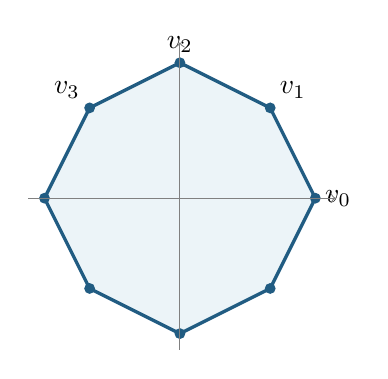
\begin{tikzpicture}[scale=1.72]
  \fill[soft] (1,0)--(2/3,2/3)--(0,1)--(-2/3,2/3)--(-1,0)--(-2/3,-2/3)--(0,-1)--(2/3,-2/3)--cycle;
  \draw[very thick,accent] (1,0)--(2/3,2/3)--(0,1)--(-2/3,2/3)--(-1,0)--(-2/3,-2/3)--(0,-1)--(2/3,-2/3)--cycle;
  \fill[accent] (1,0) circle (0.04);
  \fill[accent] (2/3,2/3) circle (0.04);
  \fill[accent] (0,1) circle (0.04);
  \fill[accent] (-2/3,2/3) circle (0.04);
  \fill[accent] (-1,0) circle (0.04);
  \fill[accent] (-2/3,-2/3) circle (0.04);
  \fill[accent] (0,-1) circle (0.04);
  \fill[accent] (2/3,-2/3) circle (0.04);
  \node[right] at (1,0) {$v_0$};
  \node[above right] at (2/3,2/3) {$v_1$};
  \node[above] at (0,1) {$v_2$};
  \node[above left] at (-2/3,2/3) {$v_3$};
  \draw[->,gray] (-1.12,0)--(1.15,0);
  \draw[->,gray] (0,-1.12)--(0,1.15);
\end{tikzpicture}
\end{center}

Identify an operator $A=(a_{ij})$ with
$z=(a_{11},a_{12},a_{21},a_{22})\in\mathbb R^4$. Since $B$ is the
convex hull of $V_+\cup -V_+$, the operator unit ball is exactly
\[
 K=B_{\Lop(X,X)}=
 \{A:f(Av)\le1\ \text{for every }v\in V_+,\ f\in\mathcal F\}. \tag{2}
\]
This is a full-dimensional rational polytope cut out by $4\cdot8=32$
half-spaces.

Let $G$ be the eight signed permutation matrices. Each element of $G$ is an
isometry of $X$, and $G\times G$ acts on $K$ by
$(U,W)\cdot A=UAW$.

\begin{lemma}[Exact vertex certificate]\label{lem:certificate}
The polytope $K$ has exactly 96 vertices. Under the $G\times G$ action they
form six orbits, represented in Table~\ref{tab:orbits}.
\end{lemma}

\subsection*{Why the enumeration is exhaustive}

For $v=(v_1,v_2)$ and $f=(f_1,f_2)$, the inequality in (2) has normal
\[
 (f_1v_1,f_1v_2,f_2v_1,f_2v_2)\in\mathbb Q^4. \tag{3}
\]
Every vertex of a full-dimensional polytope in $\mathbb R^4$ has four
linearly independent active inequalities. We therefore examine all
\(\binom{32}{4}=35{,}960\) four-subsets of the normals (3). For each subset,
exact Gauss--Jordan elimination over $\mathbb Q$ either detects dependence or
returns its unique intersection. Retaining precisely the intersections that
satisfy all 32 inequalities gives 96 distinct points. Conversely, every
retained point is the unique feasible intersection of four independent
supporting hyperplanes, hence is a vertex. Exact signed-permutation orbit
closure yields sizes
\[
 8,\ 8,\ 16,\ 16,\ 16,\ 32,
\]
and the six rational representatives in Table~\ref{tab:orbits}. This proves
Lemma~\ref{lem:certificate}. The included verifier implements exactly these
finite steps with Python's standard-library \texttt{Fraction} class; no
floating-point decision occurs.

\begin{table}[H]
\centering
\footnotesize
\renewcommand{\arraystretch}{1.08}
\begin{tabular}{c c c}
\toprule
Representative $A$ & Orbit size & Vertex witness \\
\midrule
$\begin{psmallmatrix}-1&0\\0&-1\end{psmallmatrix}$
& 8 & $Av_0=-v_0$ \\
$\begin{psmallmatrix}-2/3&-2/3\\-2/3&2/3\end{psmallmatrix}$
& 8 & $Av_0=-v_1$ \\
$\begin{psmallmatrix}-1&-1/2\\0&0\end{psmallmatrix}$
& 16 & $Av_0=-v_0$ \\
$\begin{psmallmatrix}-2/3&-1/3\\-2/3&-1/3\end{psmallmatrix}$
& 16 & $Av_0=-v_1$ \\
$\begin{psmallmatrix}-3/4&-3/4\\-1/2&1/2\end{psmallmatrix}$
& 16 & $Av_1=-v_0$ \\
$\begin{psmallmatrix}-3/4&-2/3\\-1/2&2/3\end{psmallmatrix}$
& 32 & $Av_2=v_3$ \\
\midrule
Total & 96 & \\
\bottomrule
\end{tabular}
\caption{The exact $G\times G$ orbit certificate.}
\label{tab:orbits}
\end{table}

\section{Proof of the counterexample}

\begin{proof}[Proof of Theorem~\ref{thm:main}]
Extreme contractions $X\to X$ are precisely the vertices of $K$. By
Lemma~\ref{lem:certificate}, every such vertex belongs to the orbit of one of
the six matrices in Table~\ref{tab:orbits}. Each representative explicitly
maps a vertex $v_i$ to a vertex $\pm v_j$.

This property is invariant under the orbit action. Indeed, if $Av=w$ with
$v,w\in\Ext B$ and $U,W\in G$, then
\[
 (UAW)(W^{-1}v)=Uw,
\]
and both $W^{-1}v$ and $Uw$ are vertices of $B$. Therefore every extreme
contraction maps some extreme point of $B_X$ to an extreme point of $B_X$.
Thus $(X,X)$ has weak L-P property. The failure of (1) was computed after the
statement of the theorem, completing the negative answer.
\end{proof}

\section{Reproduction and novelty check}

From this packet directory, run
\begin{verbatim}
conda run --no-capture-output -n sandbox python \
  code/verify_rational_octagon_weak_lp.py
\end{verbatim}
It reports 32 constraints, 35,960 four-subsets, 96 operator vertices, zero
bad vertices, and the six symmetry orbits above.

A bounded 19 July 2026 search found the weak L-P terminology only in the 2019
introduction (arXiv:1902.06917), the source (arXiv:2006.15318), and a commented
definition in arXiv:2407.05545 within the local 35,297-paper corpus. Exact web
searches found no later answer or octagon example. Novelty confidence is
moderate--high, subject to full bibliographic review.

\end{document}
